\documentclass[15pt]{article}
\usepackage{float}	
\usepackage[margin=1in]{geometry}		% For setting margins
\usepackage{amsmath}				% For Math
\usepackage{fancyhdr}				% For fancy header/footer
\usepackage{graphicx}				% For including figure/image
\usepackage{biblatex}
\usepackage{cancel}					% To use the slash to cancel out stuff in work

%%%%%%%%%%%%%%%%%%%%%%
% Set up fancy header/footer
\pagestyle{fancy}
\fancyhead[LO,L]{Arvid Kolstad - 020814-8452, Simon Eriksson - 0201209-2316}
\fancyhead[RO,R]{FFR110 Computational biology}
\fancyfoot[LO,L]{}
\fancyfoot[CO,C]{\thepage}
\fancyfoot[RO,R]{}
\renewcommand{\headrulewidth}{0.4pt}
\renewcommand{\footrulewidth}{0.4pt}
%%%%%%%%%%%%%%%%%%%%%%


\begin{document}
\section{Problem 1}
In this text the questions for problem 1 for assignment 2 is presented, solved and answered. the system that is being analyzed in this problem is the following:
\begin{equation}
	\frac{\partial n}{\partial t} = r n \left(1 - \frac{n}{K}\right) - \frac{A n}{1 +n/B} + \frac{\partial^2 n}{\partial x^2}
\end{equation}

\subsection{a)}
For this first assignment the equation for the system is to be transformed to dimensionless parameters this is done by the following substitutions:
\begin{equation}
	\tau = At
\end{equation}
\begin{equation}
	\xi = x\sqrt{\frac{A}{D}}
\end{equation}
\begin{equation}
	u(\xi,\tau) = \frac{n(x,t)}{B}
\end{equation}
To begin the transformation we start with evaluate the following:
\begin{equation}
	\frac{\partial u}{\partial \tau} = \frac{\partial u}{\partial t}\frac{\partial t }{\partial \tau} = \frac{1}{BA}\cdot\frac{\partial n}{\partial t}
\end{equation}
\begin{equation}
	\frac{\partial^2 u}{\partial \xi^2}	 = \frac{\partial^2 u}{\partial  x ^2} \left( \frac{\partial x}{\partial xi}\right)^2 = \frac{D}{BA} \cdot \frac{\partial^2 n}{\partial x^2}
\end{equation}

With these two equations we can transform our system:
\begin{equation}
	\frac{\partial u}{\partial \tau} = \frac{1}{BA} \left( r B u (1 - \frac{Bu}{K}) - \frac{ABu}{1+u} + AB \frac{\partial^2 u}{\partial \xi ^2}\right) = \rho u (1 - \frac{u}{q}) - \frac{u}{1+u} + \frac{\partial^2 u}{\partial \xi^2}
	\label{eq:dimless system}
\end{equation}
Where $\rho = \frac{r}{A}$ and $q = \frac{K}{B}$.
\\ \\
To get the steady states of the system we set equation \ref{eq:dimless system} equal to zero and solve for u. In the question for this assignment the diffusion term is neglected because the spatially homogenous solutions is sought for.
\begin{equation}
	u\left(\rho (1 - \frac{u}{q}) - \frac{1}{1+u}\right) = 0 \implies u^*_1 = 0
\end{equation}
If u isn't zero the equation simplifies to the following:
\begin{equation}
	\rho (1 - \frac{u}{q}) - \frac{1}{1+u} = 0
\end{equation}
solving this expression for u gives the following result:
\begin{equation}
	u^*_{2,3}= \frac{1}{2}\left(q-1 \pm \sqrt{(q-1)^2 -4 q(\frac{1}{\rho} -1 )}\right)
\end{equation}
which gives the approximate answers $u^*_2 = 1.438$ and $u^*_3 = 5.562$.


\subsection{b)}
In this section we have analyzed 3 different starting positions. The function for the starting condition was the following:
\begin{equation}
	u(\epsilon, 0) = \frac{u_0}{1 + e^{\epsilon - \epsilon_0}}
\end{equation}
where the value of $u_0$ decides how high the concentration will be from zero up to $\epsilon_0$ and after a exponential decay goes down to zero. We will also try to find a traveling wave for every simulation and if one is found, the traveling velocity $c$ will be calculated and the phase plot for a given time will be shown with respect to $u$ and $v = \frac{\partial u}{\partial \xi}$. We will also calculate the stability of the stable points found in question a) given the numerically estimated value of $c$. This will be done by the taking the following system from equation \ref{eq:dimless system}:
\begin{equation}
	\frac{\partial u}{\partial \xi} = v
\end{equation}
\begin{equation}
	\frac{\partial v}{\partial \xi} = \frac{u}{1+u} - \rho u (1-\frac{u}{q}) + \frac{\partial u}{\partial \tau}
	\label{eq:dvdxi before sub}
\end{equation}
The transformation for a traveling wave to stand still is given by $z = \xi - ct$ where $c$ is the wave velocity, and with this we can do the following substitutions:
\begin{equation}
	\frac{\partial u}{\partial \tau} = \frac{\partial u}{\partial z} \frac{\partial z}{\partial \tau} = -c\frac{\partial u}{\partial z}
\end{equation}
\begin{equation}
	\frac{\partial u}{\partial \xi} = \frac{\partial u}{\partial z} \frac{\partial z}{\partial \xi} = \frac{\partial u}{\partial z} = v
\end{equation}
This means that equation \ref{eq:dvdxi before sub} becomes:
\begin{equation}
	\frac{\partial v}{\partial \xi} = \frac{u}{1+u} - \rho u (1-\frac{u}{q}) -cv
\end{equation}

The jacobian of this system therefore becomes:
\begin{equation}
	J = \begin{pmatrix}
		0                                                   & 1  \\
		\frac{1}{(u+1)^2} - \rho\left(1- \frac{u}{q}\right) & -c
	\end{pmatrix}
\end{equation}
and solving the eigenvalues for this matrix generates the following equation for the eigenvalues:
\begin{equation}
	\lambda_{1,2} = \frac{1}{2}\left( -c \pm \sqrt{c^2 + 4 \left(\frac{1}{(1+u)^2} - \rho(1-\frac{2u}{q})\right)}\right)
	\label{eq:eigenvalues}
\end{equation}

\subsubsection{i)}
In figure \ref{fig:b11} we can see the the first simlulation. We can see that quickly forms a traveling wave that goes to the right where the concentration is rising from $u^*_1$ to $u^*_3$. In figure \ref{fig:b12} we calculated the wave velocity to $c = 0.181$. Substitution with numerical values for $u = u^*_1$ and $u= u^*_3$ in equation \ref{eq:eigenvalues}, we get that the the eigenvalues are real-valued with a negative and a positive value. This therefore means that the classification of the stable points are both saddle-points.
\begin{figure}[H]
	\begin{center}
		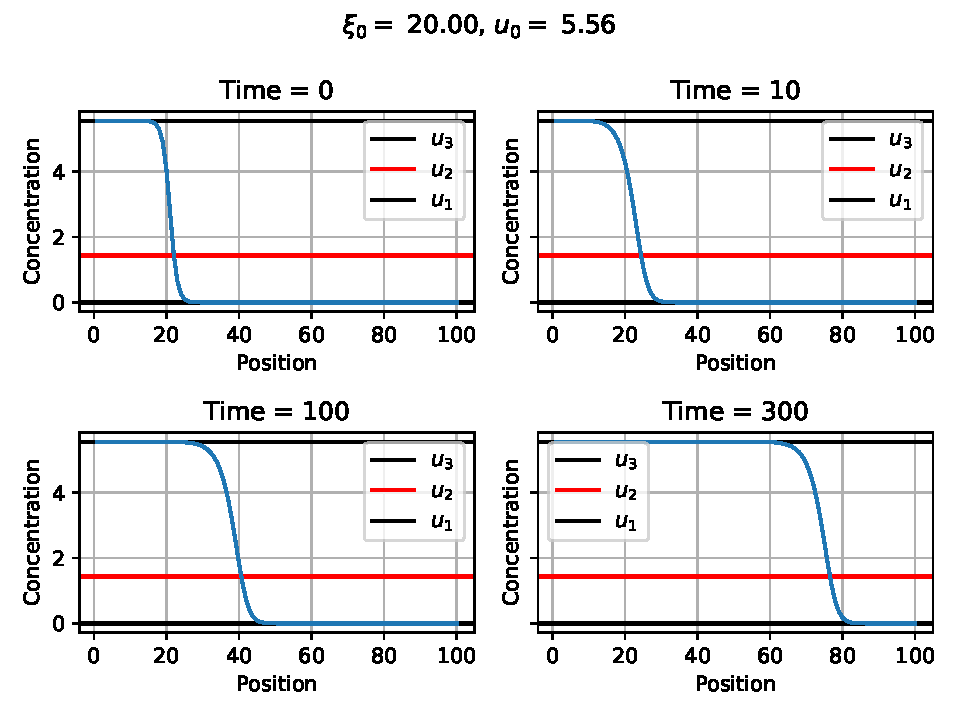
\includegraphics[width=0.70\textwidth]{figures/1b1.pdf}
	\end{center}
	\caption{Figure over different time steps of the simulation with the first starting configuration.}\label{fig:b11}
\end{figure}

\begin{figure}[H]
	\begin{center}
		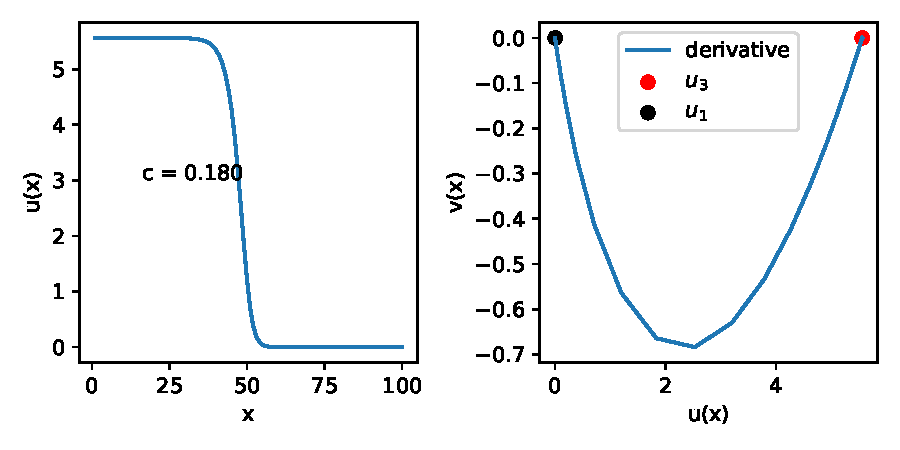
\includegraphics[width=0.70\textwidth]{figures/1b1standingwave.pdf}
	\end{center}
	\caption{Figure over the trajectory of the traveling wave and the phase plot of the same trajectory. }\label{fig:b12}
\end{figure}
\subsubsection{ii)}
In figure \ref{fig:b21} we see different time step over the simulation done with the second starting condition. We see in the figure that it slowly decays from the unstable concentration $u_2$ to the stable concentration $u_1$ from the left. In figure \ref{fig:b22} we calculated the final wave velocity to be $-0.633$ and paired with the values of the stable points it was calculated that the eigenvalues for $u_1$ was two real-values with opposite sign, which means a saddle-point and for the $u_2$ it was a complex number with both two positive real parts which mean that the stable point is a unstable spiral.

\begin{figure}[H]
	\begin{center}
		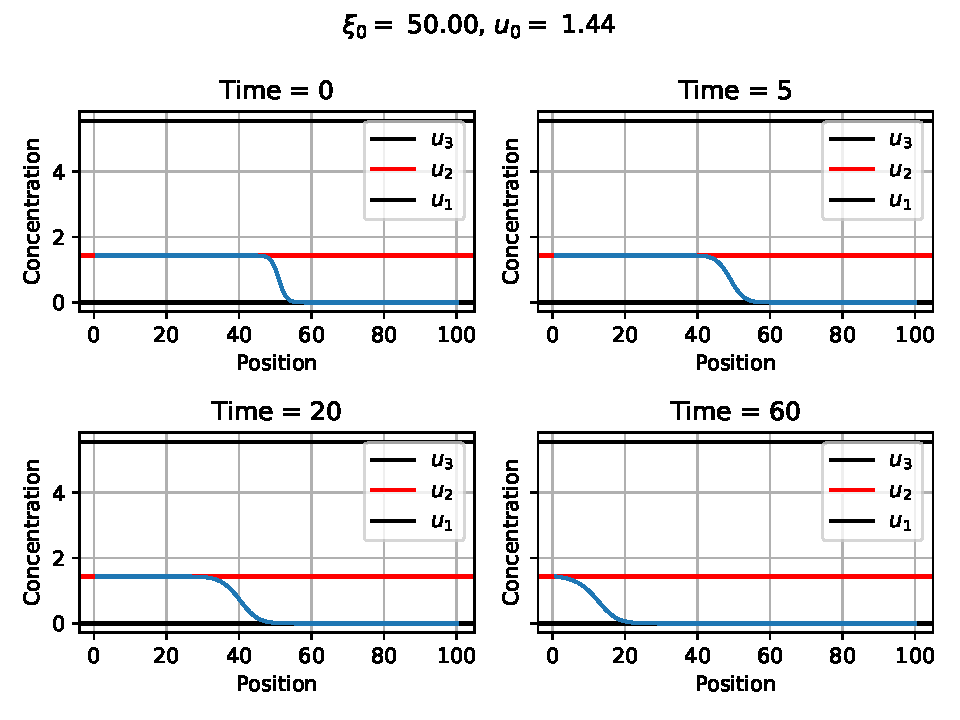
\includegraphics[width=0.70\textwidth]{figures/1b2.pdf}
	\end{center}
	\caption{Figure over the simulation with the second starting configuration.}\label{fig:b21}
\end{figure}
\begin{figure}[H]
	\begin{center}
		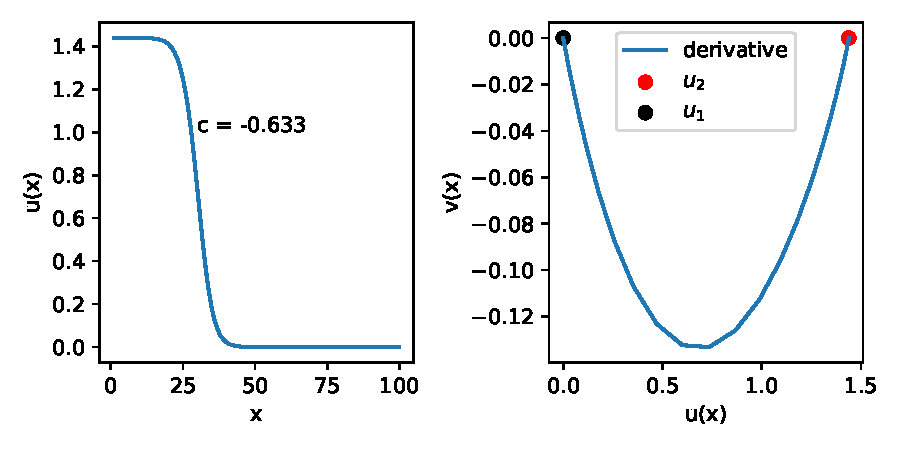
\includegraphics[width=0.70\textwidth]{figures/1b2standingwave.pdf}
	\end{center}
	\caption{Figure over the trajectory of the traveling wave and the phase plot of the same trajectory.}\label{fig:b22}
\end{figure}

\subsubsection{iii)}
In figure \ref{fig:b31} we see the simulation of the third starting configuration. We see that between $t = 0$ and $t = 40$ the left side grows from $u^*_2$ towards $u^*_3$ and then creates a traveling wave after this, similar to the first starting configuration. And as we can se in figure \ref{fig:b32} we get the same wave velocity $c= 0.181$ which therefore tells us that we get the same eigenvalues and therefore the same classification, two saddle-points.

\begin{figure}[H]
	\begin{center}
		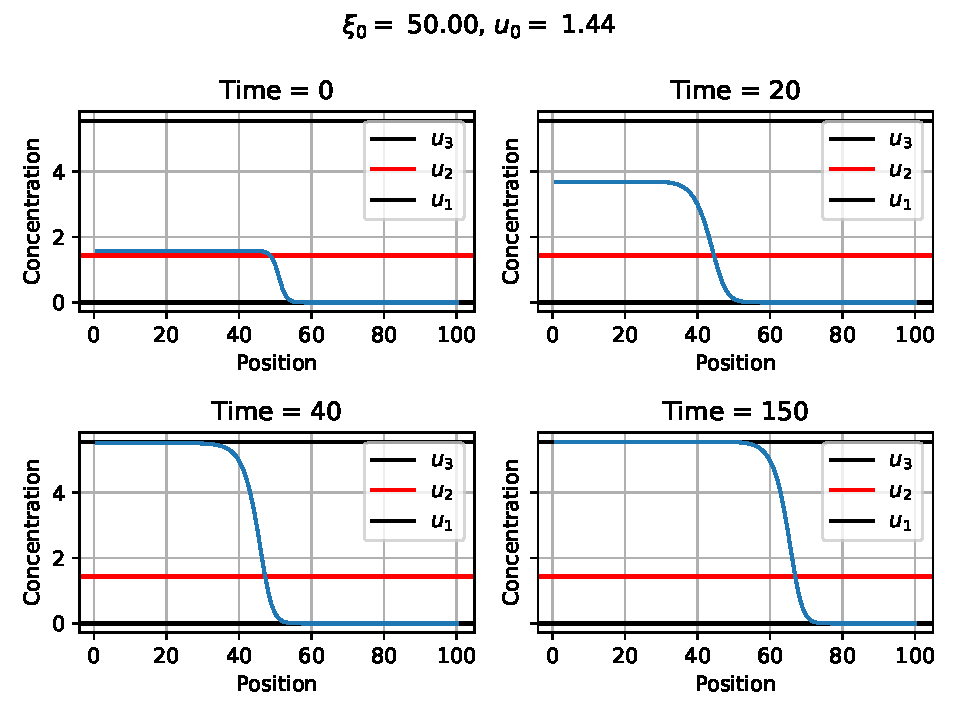
\includegraphics[width=0.70\textwidth]{figures/1b3.pdf}
	\end{center}
	\caption{Figure over the simulation of the third starting configuration.}\label{fig:b31}
\end{figure}
\begin{figure}[H]
	\begin{center}
		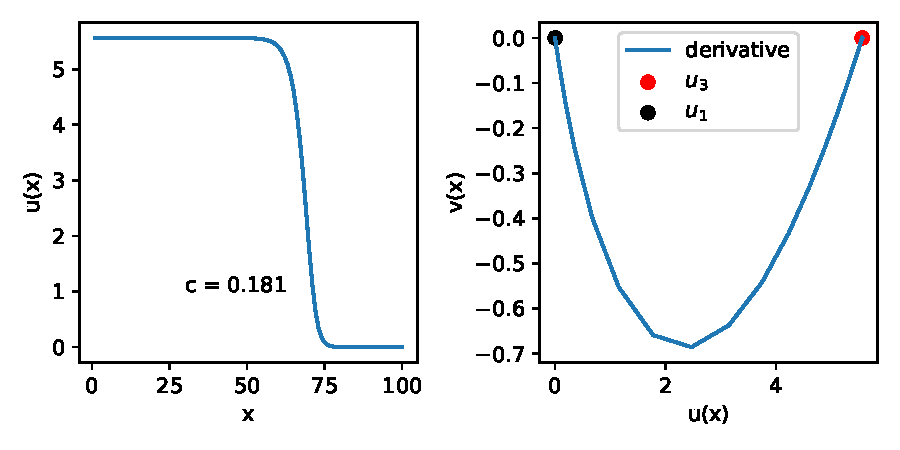
\includegraphics[width=0.70\textwidth]{figures/1b3standingwave.pdf}
	\end{center}
	\caption{Figure over a trajectory of a traveling wave from the simulation and the phase plot over the same trajectory.}\label{fig:b32}
\end{figure}

\section{c)}
In this section we switch the configuration to the following equation instead:
\begin{equation}
	u(\xi, 0)= u_0 e^{-(\xi - \xi_0)^2}
\end{equation}
This equation creates, as can be seen in figure \ref{fig:c1} and \ref{fig:c2} a much smaller starting configuration centered around $\epsilon_0$.

In figure \ref{fig:c1} we see the simulation of the first modified starting configuration. We can clearly see that it quickly decays and dies down to $u^*_1$ with no traveling wave being created.

\begin{figure}[H]
	\begin{center}
		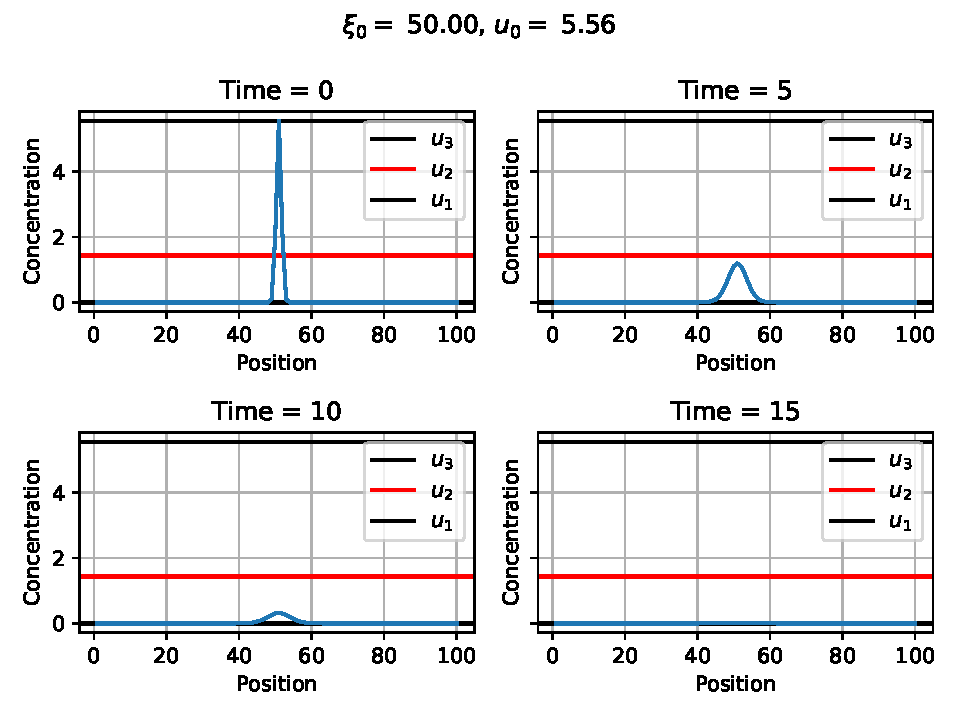
\includegraphics[width=0.70\textwidth]{figures/1c1}
	\end{center}
	\caption{Figure over the first modified starting configuration.}\label{fig:c1}
\end{figure}

In figure \ref{fig:c2} it first starts do decrease, but as it spreads it never fully goes down to $u^*_1$ but instead goes up again towards $u^*_3$. It still does not create a traveling wave because of it traveling at the same time in both directions and can therefore no be transformed to a static wave with the transformation $z= \xi -ct$.

\begin{figure}[H]
	\begin{center}
		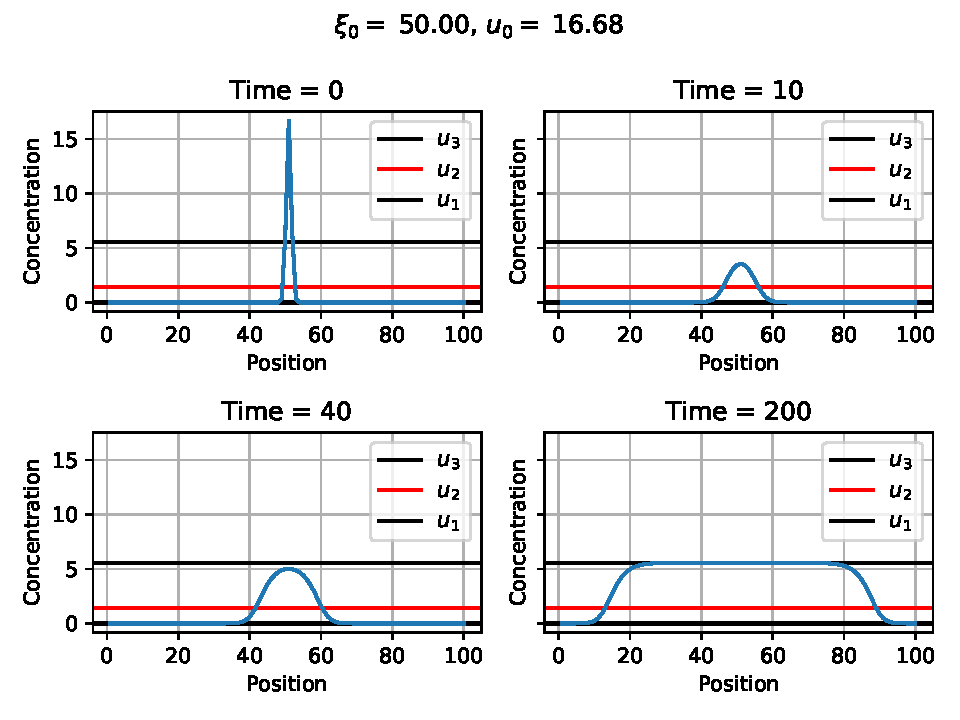
\includegraphics[width=0.70\textwidth]{figures/1c2.pdf}
	\end{center}
	\caption{Figure over the second modified starting configuration.}\label{fig:c2}
\end{figure}


\section{code}
\begin{verbatim}
import numpy as np
import matplotlib.pyplot as plt


def euler_first_derivative(f, h):
    first_derivative = (np.roll(f, -1) - np.roll(f, 1)) / 2 * h
    first_derivative = np.delete(first_derivative, [0, -1])
    return first_derivative


def euler_second_derivative(f, h):
    second_derivative = (np.roll(f, -1) + np.roll(f, 1) - 2 * f) / (h**2)
    return second_derivative


def system(u: np.ndarray, rho: float, q: float, d2udxi2: np.ndarray) -> np.ndarray:
    dudt = rho * u * (1 - u / q) - u / (1 + u) + d2udxi2
    return dudt


def start_concentration(u_0: float, xi_0: float, habitat_size: int) -> np.ndarray:
    index = np.arange(0, habitat_size, dtype=int)
    start_concentration = u_0 / (1 + np.exp(index - xi_0))
    return start_concentration


def start_concentration2(u_0: float, xi_0: float, habitat_size: int) -> np.ndarray:
    index = np.arange(0, habitat_size, dtype=int)
    start_concentration = u_0 * np.exp(-((index - xi_0) ** 2))
    return start_concentration


def run_iteration(
    n_i: np.ndarray, rho: float, q: float, time_step: float, habitat_step: float = 1.0
) -> np.ndarray:
    d2dxi2 = euler_second_derivative(n_i, habitat_step)
    d2dxi2[0] = 0.0
    d2dxi2[-1] = 0.0
    dudt = system(n_i, rho, q, d2dxi2)
    n_new = dudt * time_step + n_i
    return n_new


def run_simulation(
    u_0: float,
    xi_0: float,
    rho: float,
    q: float,
    habitat_size: int,
    sim_time: int,
    time_step: float,
    second_init=False,
):
    sim_steps = int(sim_time / time_step)
    simulation_matrix = np.zeros((habitat_size, sim_steps))
    if second_init:
        simulation_matrix[:, 0] = start_concentration2(u_0, xi_0, habitat_size)
    else:
        simulation_matrix[:, 0] = start_concentration(u_0, xi_0, habitat_size)

    for idx in range(0, sim_steps - 1):
        simulation_matrix[:, idx + 1] = run_iteration(
            simulation_matrix[:, idx], rho, q, time_step
        )
    return simulation_matrix


def get_velocity_of_wave(
    simulation_matrix, u_stable, t_min, t_max, delta_step, time_step
) -> np.ndarray:
    index = np.arange(t_min, t_max, delta_step)
    c_array = np.zeros_like(index, dtype=float)

    conc_search = u_stable / 2
    for i, time in enumerate(index):
        x_min = np.abs(simulation_matrix[20:, time] - conc_search).argmin()
        x_max = np.abs(simulation_matrix[20:, time + delta_step] - conc_search).argmin()

        c_array[i] = ((x_max - x_min) / (delta_step)) / time_step
    return c_array


def plot1():
    rho = 0.5
    q = 8.0
    u_01 = 1 / 2 * (q - 1 + np.sqrt((q - 1) ** 2 - 4 * q * (1 / rho - 1)))
    u_02 = 1 / 2 * (q - 1 - np.sqrt((q - 1) ** 2 - 4 * q * (1 / rho - 1)))

    xi_0 = 20
    time_step = 0.1
    habitat_step = 1
    sim_time = 1000
    habitat_size = 100

    sim_matrix = run_simulation(u_01, xi_0, rho, q, habitat_size, sim_time, time_step)

    plot_steps = np.array([0, 100, 1000, 3000])
    x = np.arange(1, habitat_size + 1, 1)
    fig, ax = plt.subplots(2, 2, sharey=True)
    ax = ax.flatten()

    for idx, time in enumerate(plot_steps):
        ax[idx].axhline(u_01, label=r"$u_3$", c="black")
        ax[idx].axhline(u_02, label=r"$u_2$", c="red")
        ax[idx].axhline(0.0, label=r"$u_1$", c="black")
        ax[idx].plot(x, sim_matrix[:, time])
        ax[idx].set_xlabel("Position")
        ax[idx].set_ylabel("Concentration")
        ax[idx].set_title(f"Time = {time*time_step:.0f}")
        ax[idx].grid()
        ax[idx].legend()

    fig.suptitle(rf"$\xi_0 =$ {xi_0:.2f}, $u_0 =$ {u_01:.2f}")
    fig.tight_layout()
    fig.savefig("../report/figures/1b1.pdf")

    t_min = int(50 / time_step)
    t_max = int(250 / time_step)
    delta_step = int(0.1 / time_step)
    t_mid = int((t_max + t_min) / 2)

    c = get_velocity_of_wave(sim_matrix, u_01, t_min, t_max, delta_step, time_step)

    dudxi = euler_first_derivative(sim_matrix[:, t_mid], habitat_step)

    fig, ax = plt.subplots(1, 2, figsize=(7, 3))
    ax[0].plot(x, sim_matrix[:, t_mid])
    ax[0].text(20, 5, f"c = {np.mean(c):.3f}")
    ax[1].plot(sim_matrix[1:-1, t_mid], dudxi, label="derivative")
    ax[1].scatter(sim_matrix[1, t_mid], dudxi[0], label="start point", color="red")
    ax[1].scatter(sim_matrix[-2, t_mid], dudxi[-1], label="end point", color="black")
    ax[1].legend()

    ax[0].set_xlabel("x")
    ax[0].set_ylabel("u(x)")
    ax[1].set_xlabel("u(x)")
    ax[1].set_ylabel("v(x)")

    fig.tight_layout()
    fig.savefig("../report/figures/1b1standi3gwave.pdf")


def plot2():
    rho = 0.5
    q = 8.0
    u_01 = 1 / 2 * (q - 1 + np.sqrt((q - 1) ** 2 - 4 * q * (1 / rho - 1)))
    u_02 = 1 / 2 * (q - 1 - np.sqrt((q - 1) ** 2 - 4 * q * (1 / rho - 1)))
    xi_0 = 50.0
    time_step = 0.1
    sim_time = 1000
    habitat_size = 100
    habitat_step = 1

    sim_matrix = run_simulation(u_02, xi_0, rho, q, habitat_size, sim_time, time_step)

    plot_times = np.array([0, 50, 200, 600])
    x = np.arange(1, habitat_size + 1, 1)
    fig, ax = plt.subplots(2, 2, sharey=True)
    ax = ax.flatten()

    for idx, time in enumerate(plot_times):
        ax[idx].axhline(u_01, label=r"$u_3$", c="black")
        ax[idx].axhline(u_02, label=r"$u_2$", c="red")
        ax[idx].axhline(0.0, label=r"$u_1$", c="black")
        ax[idx].plot(x, sim_matrix[:, time])
        ax[idx].set_xlabel("Position")
        ax[idx].set_ylabel("Concentration")
        ax[idx].set_title(f"Time = {time*time_step:.0f}")
        ax[idx].grid()
        ax[idx].legend()

    fig.suptitle(rf"$\xi_0 =$ {xi_0:.2f}, $u_0 =$ {u_02:.2f}")
    fig.tight_layout()
    fig.savefig("../report/figures/1b2.pdf")

    t_min = int(20 / time_step)
    t_max = int(50 / time_step)
    delta_step = int(0.1 / time_step)

    t_mid = int((t_max + t_min) / 2)

    c = get_velocity_of_wave(sim_matrix, u_02, t_min, t_max, delta_step, time_step)
    dudxi = euler_first_derivative(sim_matrix[:, t_mid], habitat_step)

    fig, ax = plt.subplots(1, 2, figsize=(10, 5))
    ax[0].plot(x, sim_matrix[:, t_mid])
    ax[0].text(30, 1, f"c = {np.mean(c):.3f}")
    ax[1].plot(sim_matrix[1:-1, t_mid], dudxi, label="derivative")
    ax[1].scatter(sim_matrix[1, t_mid], dudxi[0], label="start point", color="red")
    ax[1].scatter(sim_matrix[-2, t_mid], dudxi[-1], label="end point", color="black")
    ax[1].legend()

    ax[0].set_xlabel("x")
    ax[0].set_ylabel("u(x)")
    ax[1].set_xlabel("u(x)")
    ax[1].set_ylabel("v(x)")

    fig.tight_layout()
    fig.savefig("../report/figures/1b2standingwave.pdf")


def plot3():
    rho = 0.5
    q = 8.0
    u_01 = 1 / 2 * (q - 1 + np.sqrt((q - 1) ** 2 - 4 * q * (1 / rho - 1)))
    u_02 = 1 / 2 * (q - 1 - np.sqrt((q - 1) ** 2 - 4 * q * (1 / rho - 1)))
    xi_0 = 50.0
    time_step = 0.1
    sim_time = 1000
    habitat_size = 100
    habitat_step = 1

    sim_matrix = run_simulation(
        u_02 * 1.1, xi_0, rho, q, habitat_size, sim_time, time_step
    )

    plot_times = np.array([0, 200, 400, 800])
    x = np.arange(1, habitat_size + 1, 1)
    fig, ax = plt.subplots(2, 2, sharey=True)
    ax = ax.flatten()

    for idx, time in enumerate(plot_times):
        ax[idx].axhline(u_01, label=r"$u_3$", c="black")
        ax[idx].axhline(u_02, label=r"$u_2$", c="red")
        ax[idx].axhline(0.0, label=r"$u_1$", c="black")
        ax[idx].plot(x, sim_matrix[:, time])
        ax[idx].set_xlabel("Position")
        ax[idx].set_ylabel("Concentration")
        ax[idx].set_title(f"Time = {time*time_step:.0f}")
        ax[idx].grid()
        ax[idx].legend()

    fig.suptitle(rf"$\xi_0 =$ {xi_0:.2f}, $u_0 =$ {u_02:.2f}")
    fig.tight_layout()
    fig.savefig("../report/figures/1b3.pdf")

    t_min = int(40 / time_step)
    t_max = int(300 / time_step)
    delta_step = int(0.1 / time_step)

    t_mid = int((t_max + t_min) / 2)

    c = get_velocity_of_wave(sim_matrix, u_01, t_min, t_max, delta_step, time_step)
    dudxi = euler_first_derivative(sim_matrix[:, t_mid], habitat_step)

    fig, ax = plt.subplots(1, 2, figsize=(10, 5))
    ax[0].plot(x, sim_matrix[:, t_mid])
    ax[0].text(30, 1, f"c = {np.mean(c):.3f}")
    ax[1].plot(sim_matrix[1:-1, t_mid], dudxi, label="derivative")
    ax[1].scatter(sim_matrix[1, t_mid], dudxi[0], label="start point", color="red")
    ax[1].scatter(sim_matrix[-2, t_mid], dudxi[-1], label="end point", color="black")
    ax[1].legend()

    ax[0].set_xlabel("x")
    ax[0].set_ylabel("u(x)")
    ax[1].set_xlabel("u(x)")
    ax[1].set_ylabel("v(x)")

    fig.tight_layout()
    fig.savefig("../report/figures/1b3standingwave.pdf")


def plot4():
    rho = 0.5
    q = 8.0
    u_01 = 1 / 2 * (q - 1 + np.sqrt((q - 1) ** 2 - 4 * q * (1 / rho - 1)))
    u_02 = 1 / 2 * (q - 1 - np.sqrt((q - 1) ** 2 - 4 * q * (1 / rho - 1)))
    xi_0 = 50.0
    time_step = 0.1
    sim_time = 1000
    habitat_size = 100

    sim_matrix = run_simulation(
        u_01, xi_0, rho, q, habitat_size, sim_time, time_step, second_init=True
    )

    plot_times = np.array([0, 50, 100, 150])
    x = np.arange(1, habitat_size + 1, 1)
    fig, ax = plt.subplots(2, 2, sharey=True)
    ax = ax.flatten()

    for idx, time in enumerate(plot_times):
        ax[idx].axhline(u_01, label=r"$u_3$", c="black")
        ax[idx].axhline(u_02, label=r"$u_2$", c="red")
        ax[idx].axhline(0.0, label=r"$u_1$", c="black")
        ax[idx].plot(x, sim_matrix[:, time])
        ax[idx].set_xlabel("Position")
        ax[idx].set_ylabel("Concentration")
        ax[idx].set_title(f"Time = {time*time_step:.0f}")
        ax[idx].grid()
        ax[idx].legend()

    fig.suptitle(rf"$\xi_0 =$ {xi_0:.2f}, $u_0 =$ {u_01:.2f}")
    fig.tight_layout()
    fig.savefig("../report/figures/1c1.pdf")


def plot5():
    rho = 0.5
    q = 8.0
    u_01 = 1 / 2 * (q - 1 + np.sqrt((q - 1) ** 2 - 4 * q * (1 / rho - 1)))
    u_02 = 1 / 2 * (q - 1 - np.sqrt((q - 1) ** 2 - 4 * q * (1 / rho - 1)))
    xi_0 = 50.0
    time_step = 0.1
    sim_time = 1000
    habitat_size = 100

    sim_matrix = run_simulation(
        u_01 * 3, xi_0, rho, q, habitat_size, sim_time, time_step, second_init=True
    )

    plot_times = np.array([0, 100, 400, 2000])
    x = np.arange(1, habitat_size + 1, 1)
    fig, ax = plt.subplots(2, 2, sharey=True)
    ax = ax.flatten()

    for idx, time in enumerate(plot_times):
        ax[idx].axhline(u_01, label=r"$u_3$", c="black")
        ax[idx].axhline(u_02, label=r"$u_2$", c="red")
        ax[idx].axhline(0.0, label=r"$u_1$", c="black")
        ax[idx].plot(x, sim_matrix[:, time])
        ax[idx].set_xlabel("Position")
        ax[idx].set_ylabel("Concentration")
        ax[idx].set_title(f"Time = {time*time_step:.0f}")
        ax[idx].grid()
        ax[idx].legend()

    fig.suptitle(rf"$\xi_0 =$ {xi_0:.2f}, $u_0 =$ {u_01 *3:.2f}")
    fig.tight_layout()
    fig.savefig("../report/figures/1c2.pdf")


def main():
    plot1()
    plot2()
    plot3()
    plot4()
    plot5()


if __name__ == "__main__":
    main()
\end{verbatim}
\end{document}
